% !TEX root = learner4_block_diagram_simple.tex
% Simple main-block diagram for Learner 4.
% Build: ./scripts/build_learner4_block_diagram.sh

\documentclass[11pt]{article}
\usepackage[landscape,margin=0.55in]{geometry}
\usepackage{amsmath,amssymb}
\usepackage{tikz}
\usetikzlibrary{positioning,arrows.meta,calc,fit}
\usepackage{xcolor}

\definecolor{handc}{RGB}{180,95,30}
\definecolor{plantc}{RGB}{140,30,40}
\definecolor{ekfc}{RGB}{27,54,93}
\definecolor{schedc}{RGB}{30,107,58}
\definecolor{failc}{RGB}{130,50,140}
\definecolor{scorec}{RGB}{70,70,70}
\definecolor{arrowgrey}{RGB}{70,70,70}

\begin{document}
\thispagestyle{empty}
\begin{center}
{\Large\bfseries Learner~4 --- one-trial flow}\\[0.2em]
{\small Same hand command $u$ drives the true plant and the EKF model;
learning updates the belief so $\hat y$ tracks $y$.}\\[0.7em]
\end{center}

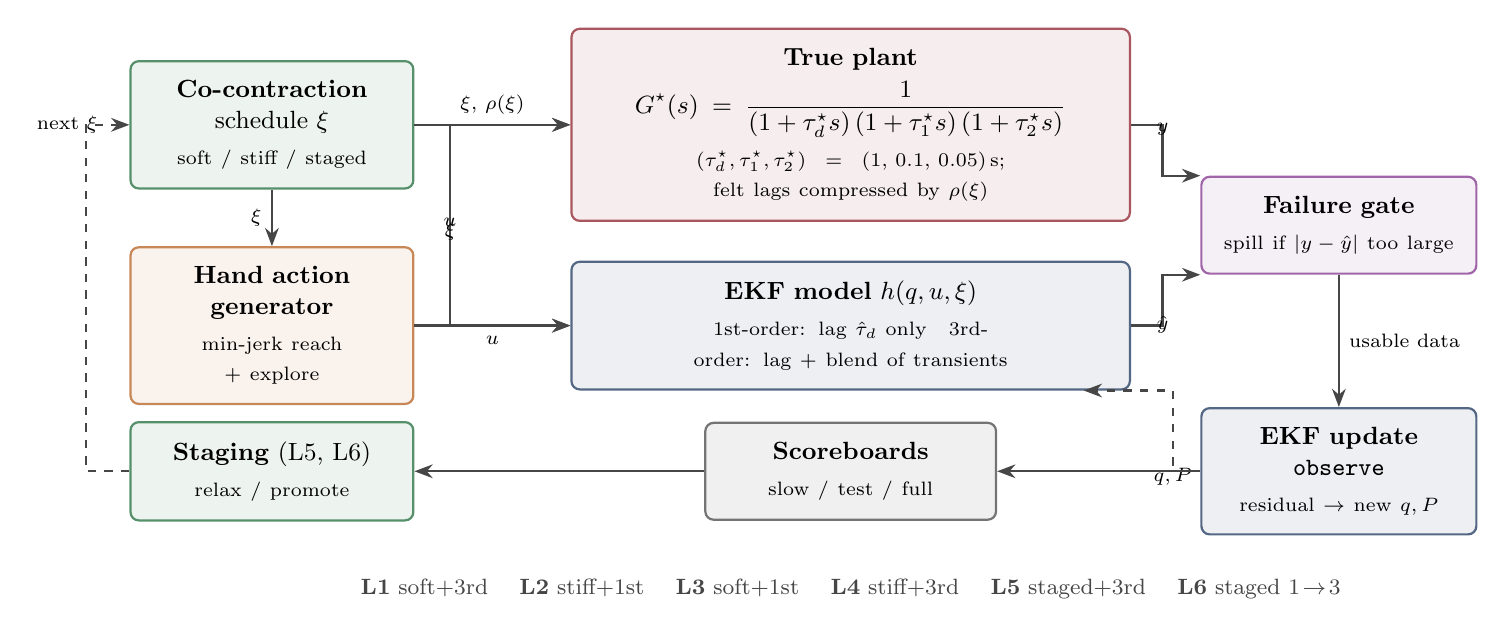
\begin{tikzpicture}[
  >=Stealth,
  font=\small,
  blk/.style 2 args={
    rectangle, rounded corners=3pt, draw=#1!75, fill=#1!8,
    thick, align=center, inner sep=7pt, text width=#2
  },
  arr/.style={->, thick, draw=arrowgrey},
  darr/.style={->, thick, draw=arrowgrey, dashed},
]

% ---- left column: grip then hand ----
\node[blk={schedc}{3.1cm}] (sched) at (0, 2.55)
  {\textbf{Co-contraction}\\ schedule $\xi$\\[2pt]
   {\scriptsize soft / stiff / staged}};

\node[blk={handc}{3.1cm}] (hand) at (0, 0)
  {\textbf{Hand action generator}\\[2pt]
   {\scriptsize min-jerk reach + explore}};

% ---- parallel plant / model ----
\node[blk={plantc}{6.6cm}] (plant) at (7.35, 2.55)
  {\textbf{True plant}\\[3pt]
   $\displaystyle G^\star(s)=\frac{1}{(1+\tau_d^\star s)\,(1+\tau_1^\star s)\,(1+\tau_2^\star s)}$\\[4pt]
   {\scriptsize $(\tau_d^\star,\tau_1^\star,\tau_2^\star)=(1,\,0.1,\,0.05)$\,s;
   felt lags compressed by $\rho(\xi)$}};

\node[blk={ekfc}{6.6cm}] (model) at (7.35, 0)
  {\textbf{EKF model} $h(q,u,\xi)$\\[2pt]
   {\scriptsize 1st-order: lag $\hat\tau_d$ only\quad
    3rd-order: lag + blend of transients}};

% ---- right column: gate then update ----
\node[blk={failc}{3.0cm}] (fail) at (13.55, 1.275)
  {\textbf{Failure gate}\\[2pt]
   {\scriptsize spill if $|y-\hat y|$ too large}};

\node[blk={ekfc}{3.0cm}] (update) at (13.55, -1.85)
  {\textbf{EKF update}\\ \texttt{observe}\\[2pt]
   {\scriptsize residual $\to$ new $q,P$}};

% ---- bottom: scoreboards / staging ----
\node[blk={scorec}{3.2cm}] (score) at (7.35, -1.85)
  {\textbf{Scoreboards}\\[2pt]
   {\scriptsize slow / test / full}};

\node[blk={schedc}{3.1cm}] (stage) at (0, -1.85)
  {\textbf{Staging} (L5, L6)\\[2pt]
   {\scriptsize relax / promote}};

% ---- arrows: left column ----
\draw[arr] (sched) -- (hand) node[midway, left, font=\scriptsize] {$\xi$};

% u splits to plant (above) and model (same height)
\draw[arr] (hand.east) -- ++(0.45,0) |- (plant.west)
  node[pos=0.22, above, font=\scriptsize] {$u$};
\draw[arr] (hand.east) -- (model.west)
  node[midway, below, font=\scriptsize] {$u$};

% xi to plant (rho) and to EKF model
\draw[arr] (sched.east) -- (plant.west)
  node[midway, above, font=\scriptsize] {$\xi,\,\rho(\xi)$};
\draw[arr] (sched.east) -- ++(0.45,0) |- (model.west)
  node[pos=0.22, below, font=\scriptsize] {$\xi$};

% plant / model to failure gate
\draw[arr] (plant.east) -- ++(0.4,0) |- (fail.north west)
  node[pos=0.2, above, font=\scriptsize] {$y$};
\draw[arr] (model.east) -- ++(0.4,0) |- (fail.south west)
  node[pos=0.2, below, font=\scriptsize] {$\hat y$};

% gate to update, update back to model
\draw[arr] (fail) -- (update)
  node[midway, right, font=\scriptsize] {usable data};
\draw[darr] (update.west) -- ++(-0.35,0) |- ($(model.south east)+(-0.6,0)$)
  node[pos=0.08, below, font=\scriptsize] {$q,P$};

% update to scoreboards and staging
\draw[arr] (update) -- (score);
\draw[arr] (score) -- (stage);
\draw[darr] (stage.west) -- ++(-0.55,0) |- (sched.west)
  node[pos=0.75, left, font=\scriptsize] {next $\xi$};

% ---- conditions ----
\node[font=\footnotesize, text=arrowgrey, align=center]
  at (7.35, -3.35)
  {\textbf{L1} soft+3rd \quad
   \textbf{L2} stiff+1st \quad
   \textbf{L3} soft+1st \quad
   \textbf{L4} stiff+3rd \quad
   \textbf{L5} staged+3rd \quad
   \textbf{L6} staged $1\!\to\!3$};

\end{tikzpicture}
\end{document}
